\subsection{Integrations}

\begin{itemize}
\item MARBL
\item ARES
\item AMRex: Warpx, Pele, NYX
\item SW4
\end{itemize}



\subsection{MARBL:Big Laser Tiny Box}
\fix{Placeholder text.}
Figures~\ref{img:radkh} and \ref{img:radkh_xray} show images create from
a simulation of a real work experiment, where scientists destroyed a tiny box
with a powerful laser.
%
This is a important use case due to the impending tiny box invasion.

\begin{figure}
\centering
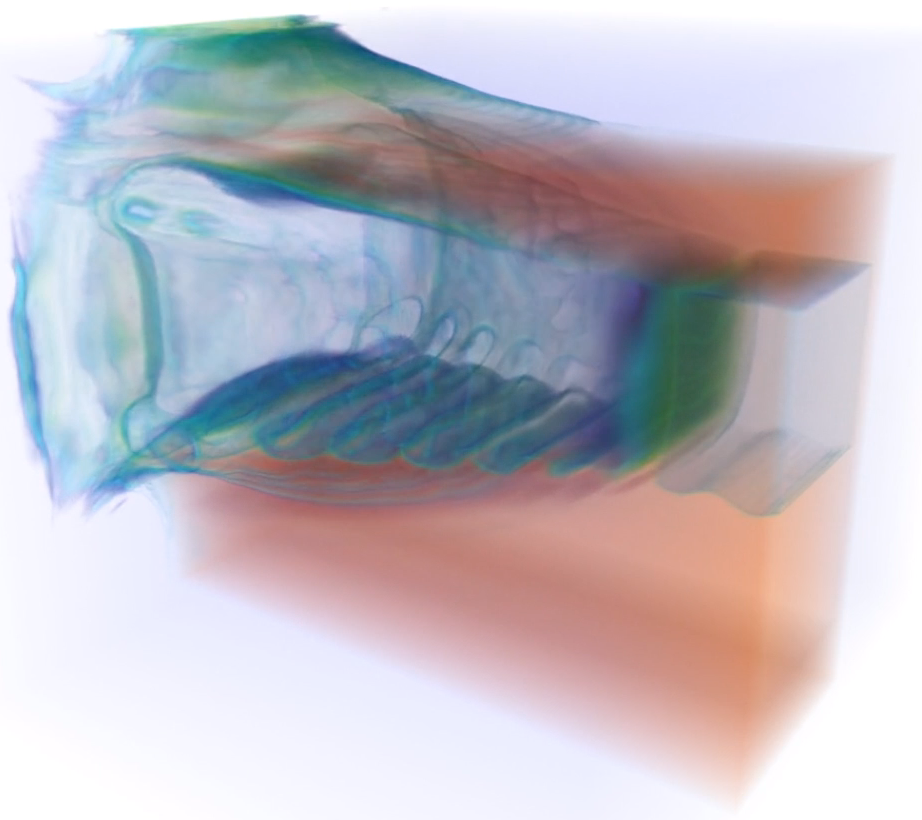
\includegraphics[width=0.6\textwidth]{images/radkh}
\caption{\label{img:radkh} Image of a comically sized lazer destroying a small box.}
\end{figure}

\begin{figure}
\centering
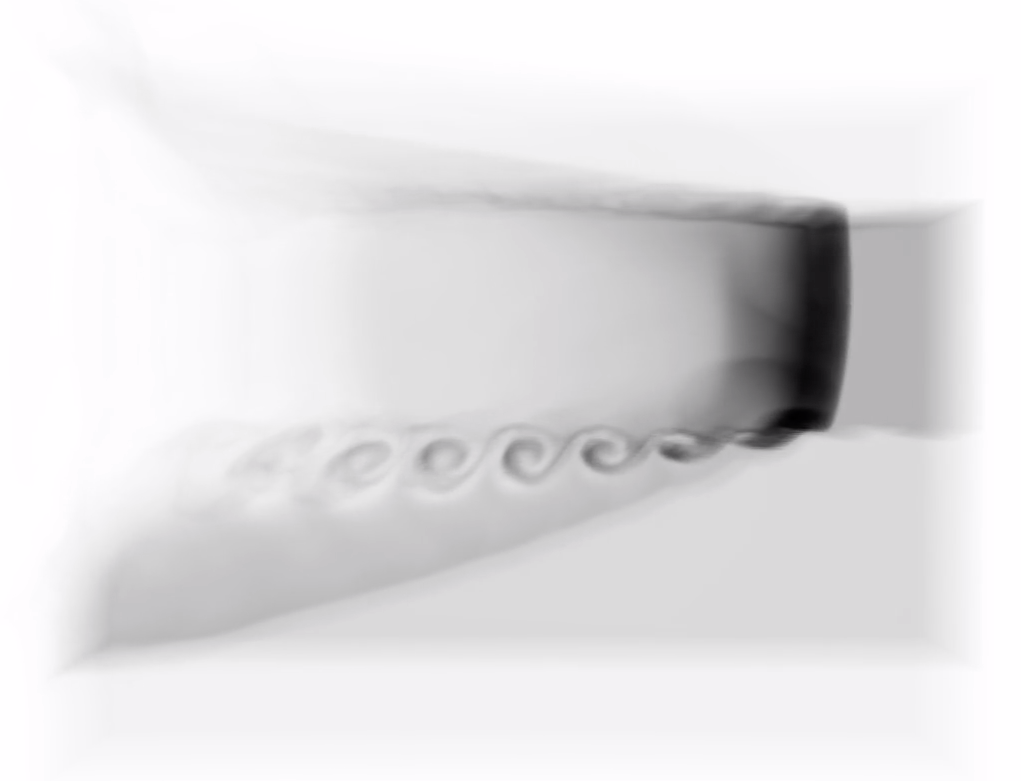
\includegraphics[width=0.6\textwidth]{images/radkh_xray}
\caption{\label{img:radkh_xray}Simulated radiograph of a comically sized lazer destroying a small box.}
\end{figure}

\subsection{In situ visualization of an Inertial Confinement Fusion (ICF) simulation}

Ascent was used to visualize the results of an unprecedented 3D simulation
of two-fluid mixing in a spherical geometry to better understand hydrodynamic
instability and the transition to turbulence process that is important to
the field of inertial confinement fusion and High Energy Density (HED)
Physics. High resolution simulations of instability growth are not practical
for routine use, so high resolution simulations like this help guide the
development of sub-grid models that capture instability effects with much
less computational cost, which are used for ICF calculations.

The simulation was run on the Lawrence Livermore National Laboratories
Sierra system, a 125 Petaflop peak system from IBM that has 4,320 nodes,
each with 2 IBM POWER9 processors, 4 NVIDIA Tesla V100 GPUs, 320 GiB of
fast memory (256 GiB DDR4 memory and 64 GiB HBM4), and 1.6TB of NVMe
memory. The specific simulation was a 97.8 billion element simulation
run across 16,384 GPUs on 4,096 compute nodes. The simulation application
used CUDA via RAJA to run on the GPUs. The time-varying evolution of the
mixing was visualized in situ with Ascent, also leveraging 16,384 GPUs.
The last time step was also exported by Ascent to the parallel file
system for detailed post-hoc visualization using VisIt. The simulation
data was accessed by Ascent directly from the GPU memory, eliminating any
extra data copies.

\begin{figure}
\centering
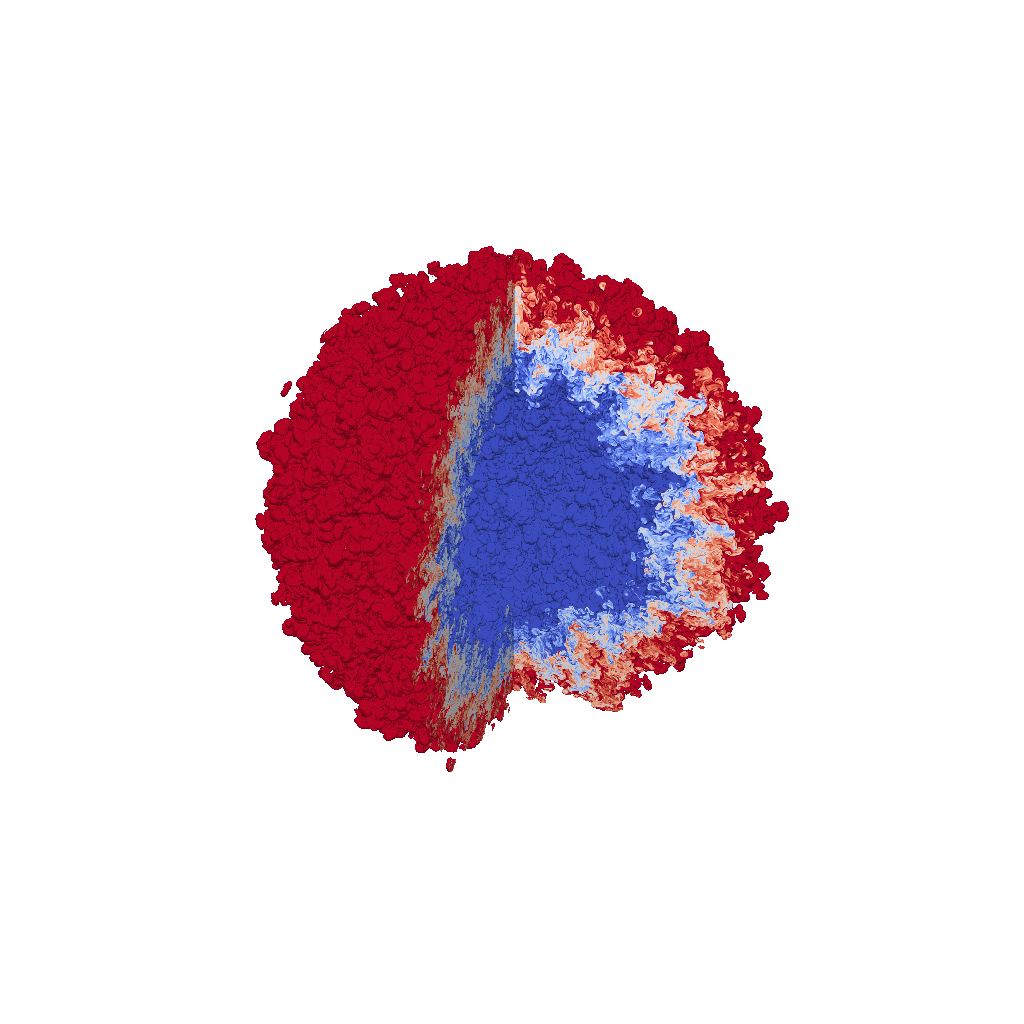
\includegraphics[trim={ 0 8cm 0 7cm},width=0.9\textwidth]{images/mixing_ball}
\caption{\label{img:icf}
This image is of an idealized Inertial Confinement
Fusion (ICF) simulation of a Rayleigh–Taylor instability
with two fluids mixing in a spherical geometry.
}
\end{figure}
